%
\hsection{Installing LibreOffice under Ubuntu Linux}%
%
\begin{figure}%
\centering%
%
\subfloat[][%
Open a terminal via with \ubuntuTerminal, then type \bashil{libreoffice --version} and hit~\keys{\enter}. %
On my system, \libreoffice~24.2.7.2 is installed.%
\label{fig:installingLibreOfficeUbuntu1checkVersion}%
]{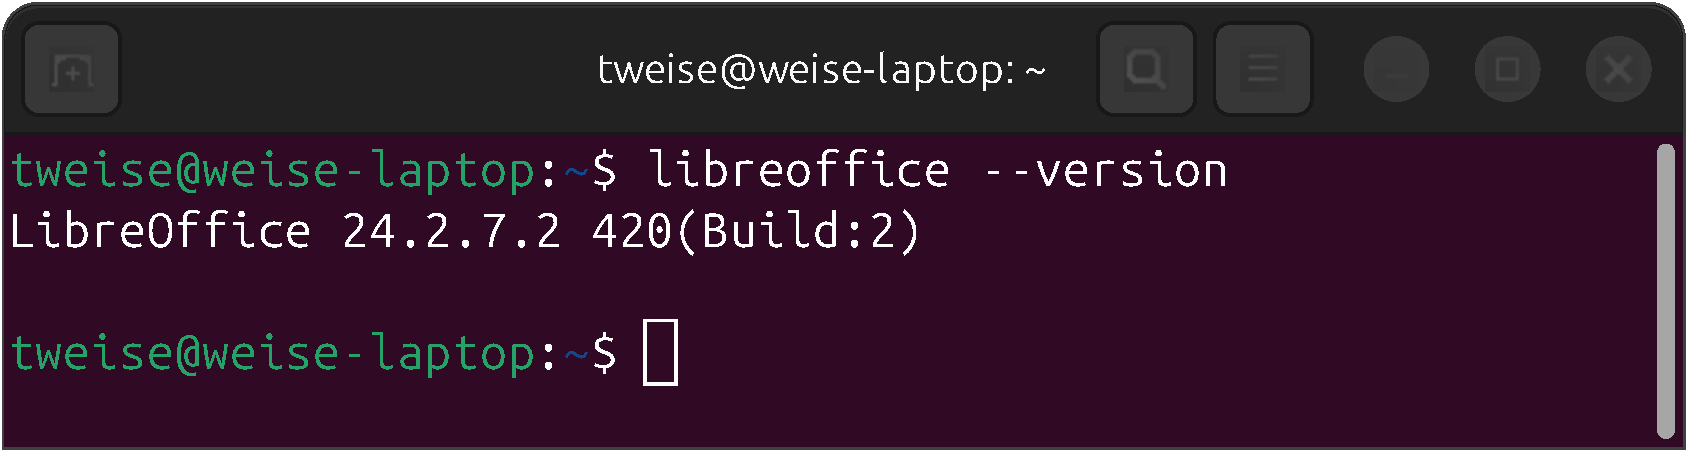
\includegraphics[width=0.7\linewidth]{\currentDir/installingLibreOfficeUbuntu1checkVersion}}%
%
\floatRowSep%
%
\subfloat[][%
We can start \libreofficeBase\ from the terminal by typing \bashil{libreoffice --base} and hitting~\keys{\enter}.%
\label{fig:installingLibreOfficeUbuntu2runFromTerminal}%
]{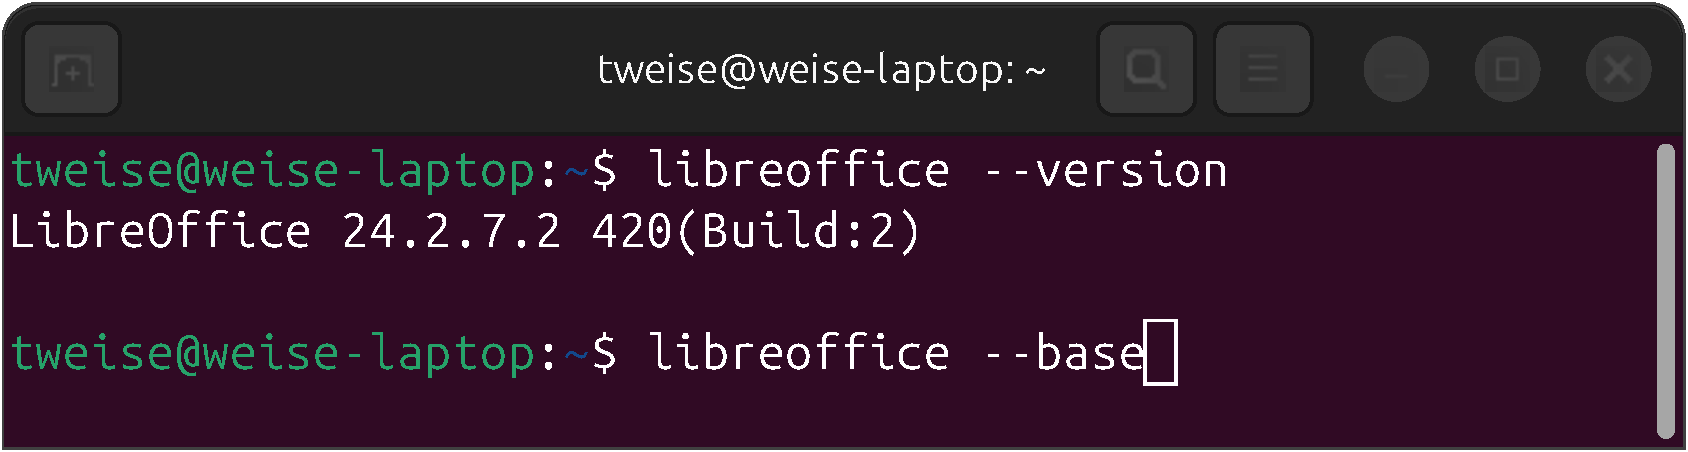
\includegraphics[width=0.7\linewidth]{\currentDir/installingLibreOfficeUbuntu2runFromTerminal}}%
%
\floatRowSep%
%
\subfloat[][%
Or we can open the dash by hitting~\keys{\OSwin}, type \textil{libreoffice}, and then clicking on the symbol for \libreofficeBase.%
\label{fig:installingLibreOfficeUbuntu4runFromDash}%
]{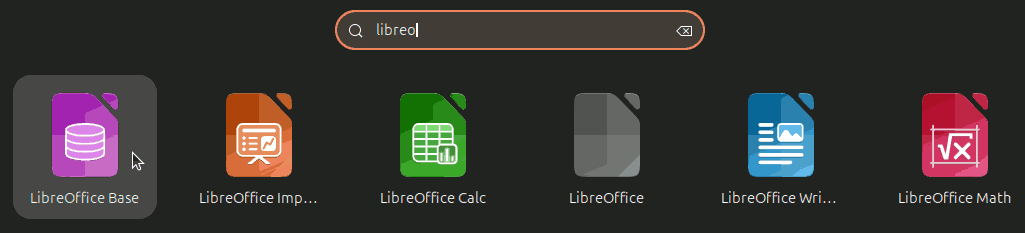
\includegraphics[width=0.65\linewidth]{\currentDir/installingLibreOfficeUbuntu4runFromDash}}%
%
\floatSep%
%
\subfloat[][%
We can also open the dash by clicking on the little \ubuntu\ symbol at the bottom-left corner of the screen.%
\label{fig:installingLibreOfficeUbuntu3openDash}%
]{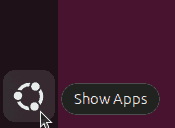
\includegraphics[width=0.33\linewidth]{\currentDir/installingLibreOfficeUbuntu3openDash}}%
%
\caption{Starting \libreofficeBase\ under \ubuntu\ if it is already installed.}%
\label{fig:installingLibreOfficeUbuntuA}%
\end{figure}%
%
\begin{figure}%
\ContinuedFloat%
\centering%
%
\subfloat[][%
The startup screen appears.%
\label{fig:installingLibreOfficeUbuntu5startupScreen}%
]{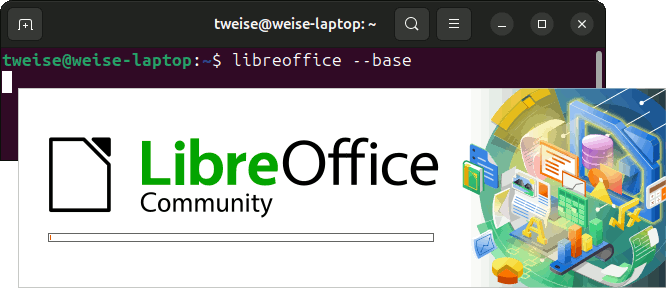
\includegraphics[width=0.8\linewidth]{\currentDir/installingLibreOfficeUbuntu5startupScreen}}%
%
\floatRowSep%
%
\subfloat[][%
The initial form of \libreofficeBase\ appears. %
We are done for now and close the program.%
\label{fig:installingLibreOfficeUbuntu6startupForm}%
]{\tightbox{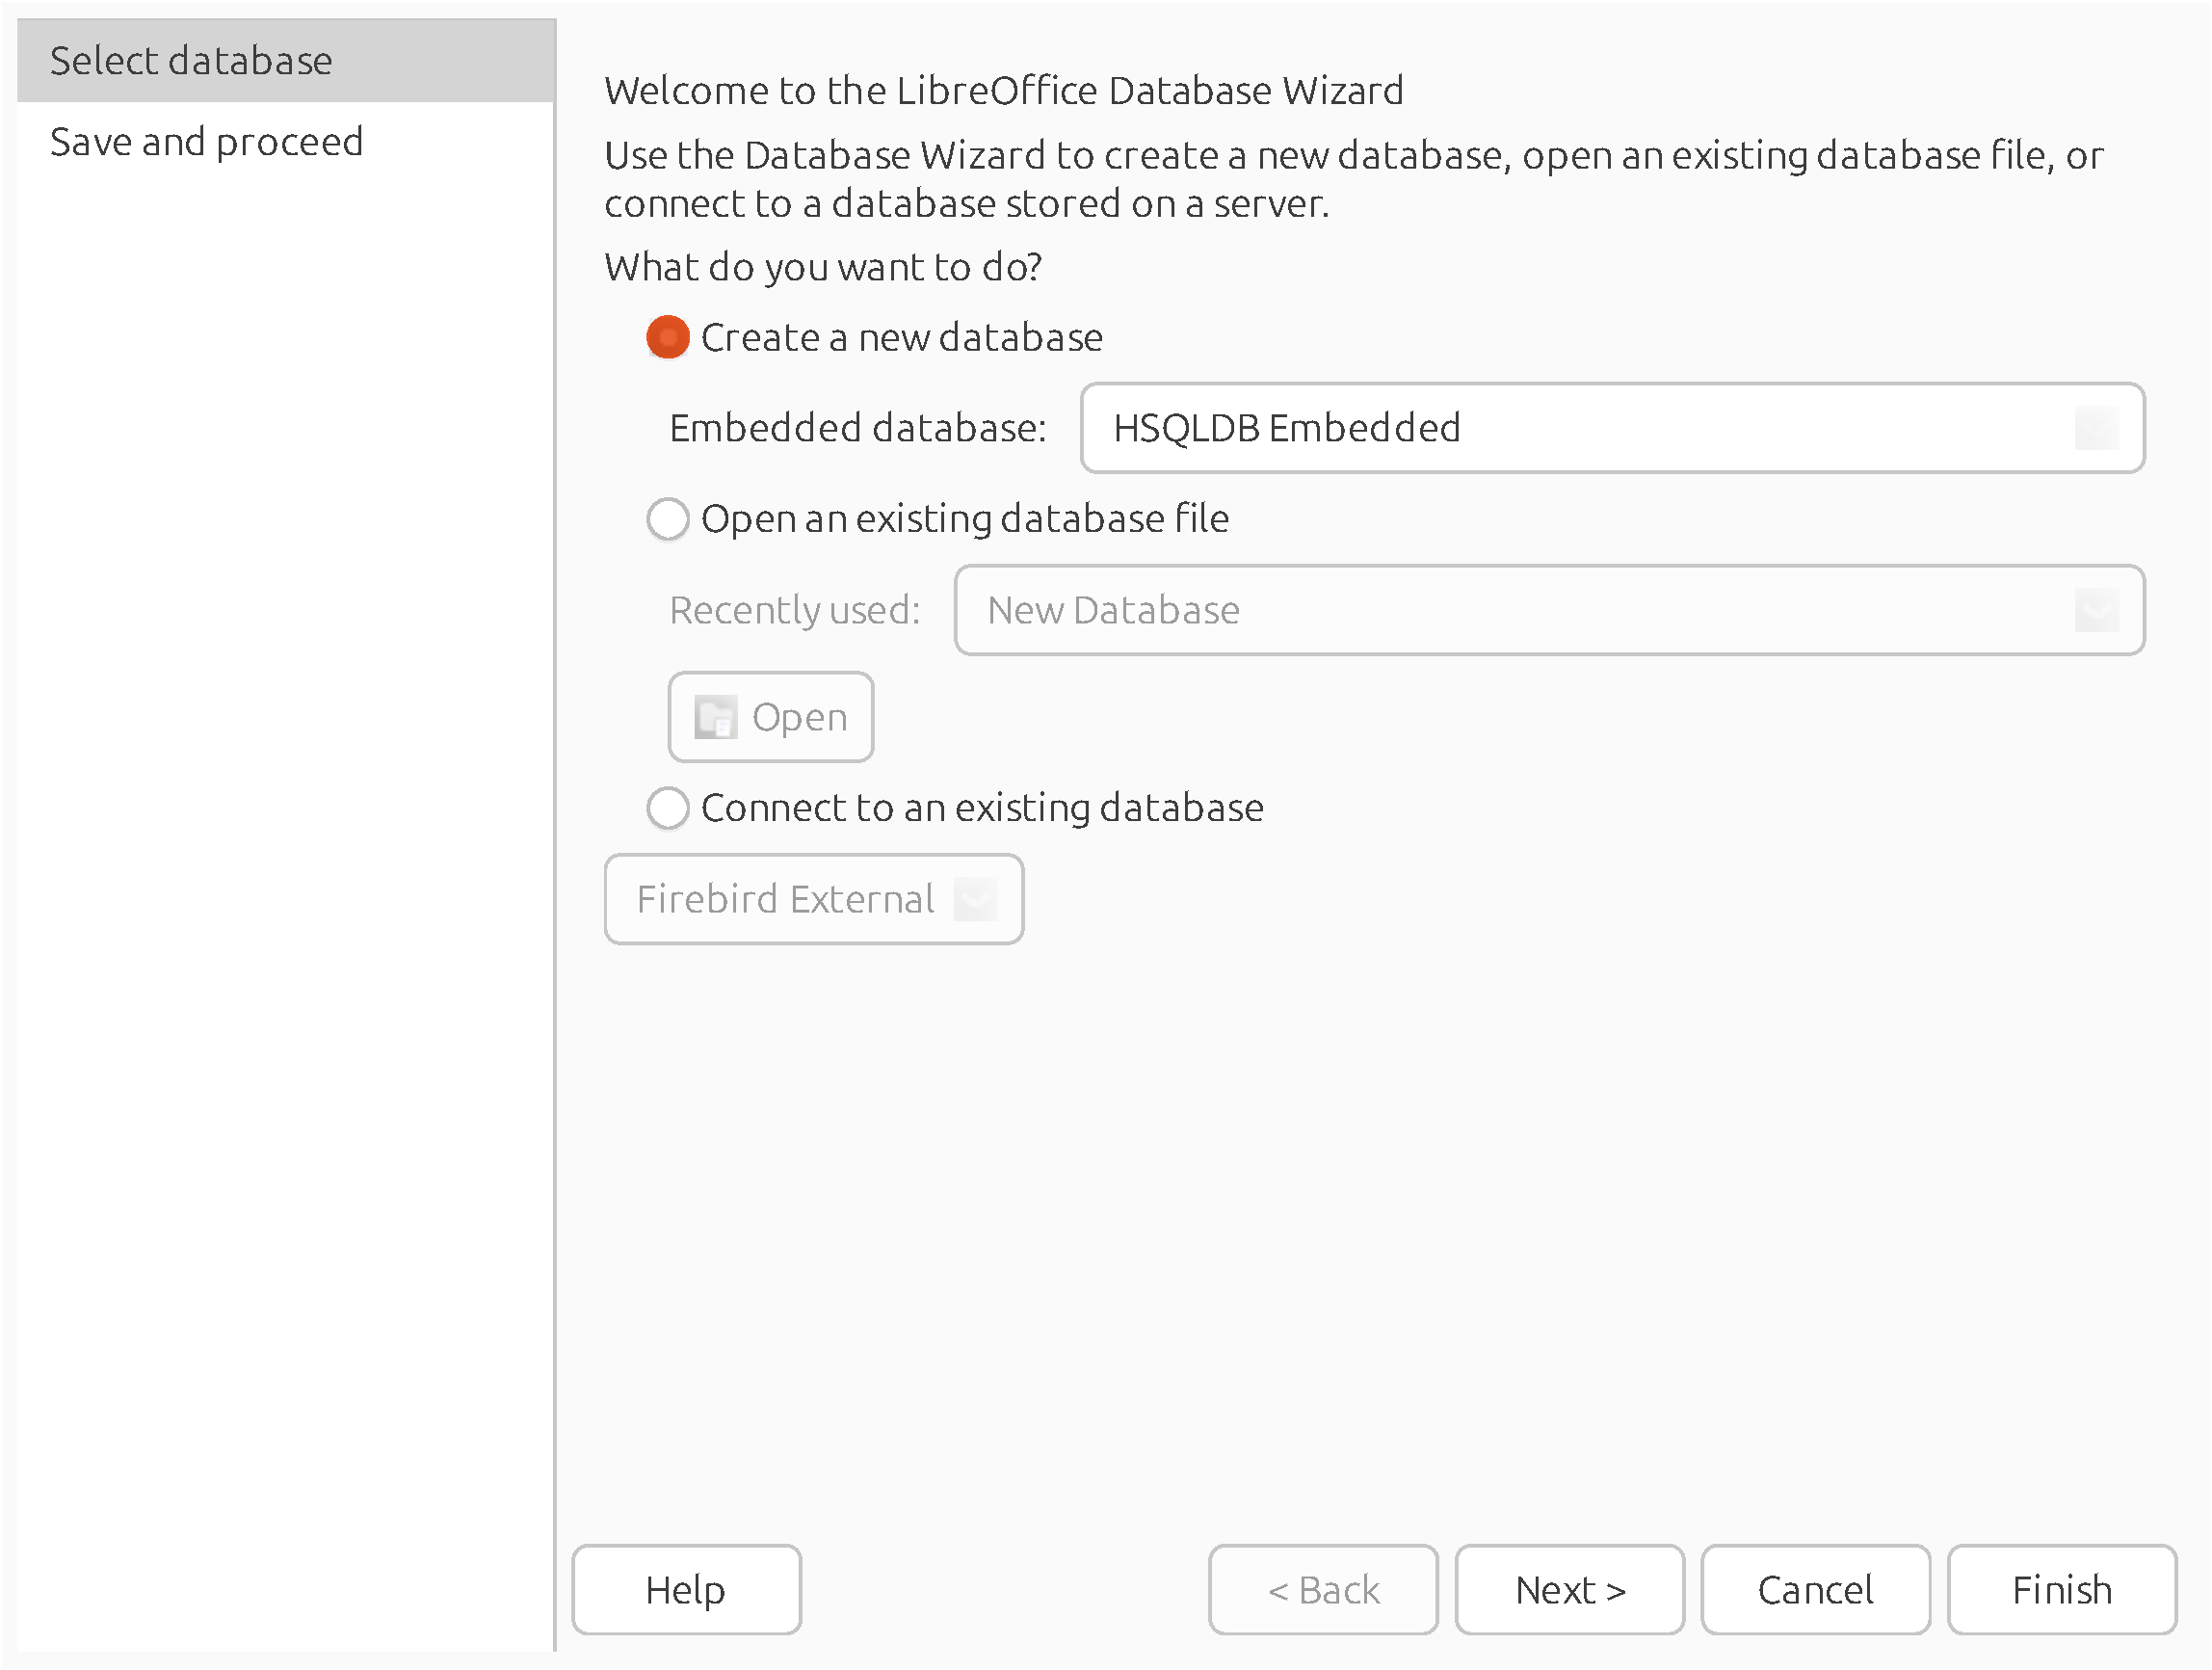
\includegraphics[width=0.8\linewidth]{\currentDir/installingLibreOfficeUbuntu6startupForm}}}%
%
\caption{Starting \libreofficeBase\ under \ubuntu\ if it is already installed.}%
\label{fig:installingLibreOfficeUbuntuB}%
\end{figure}%
%
\begin{figure}%
\centering%
%
\subfloat[][%
In the unlikely case that \libreoffice\ was not installed, we can install it by typing \bashil{sudo apt-get install libreoffice} into a terminal window that we opened with \ubuntuTerminal\ and hit~\keys{\enter}.%
\label{fig:installingLibreOfficeUbuntu7aptGet}%
]{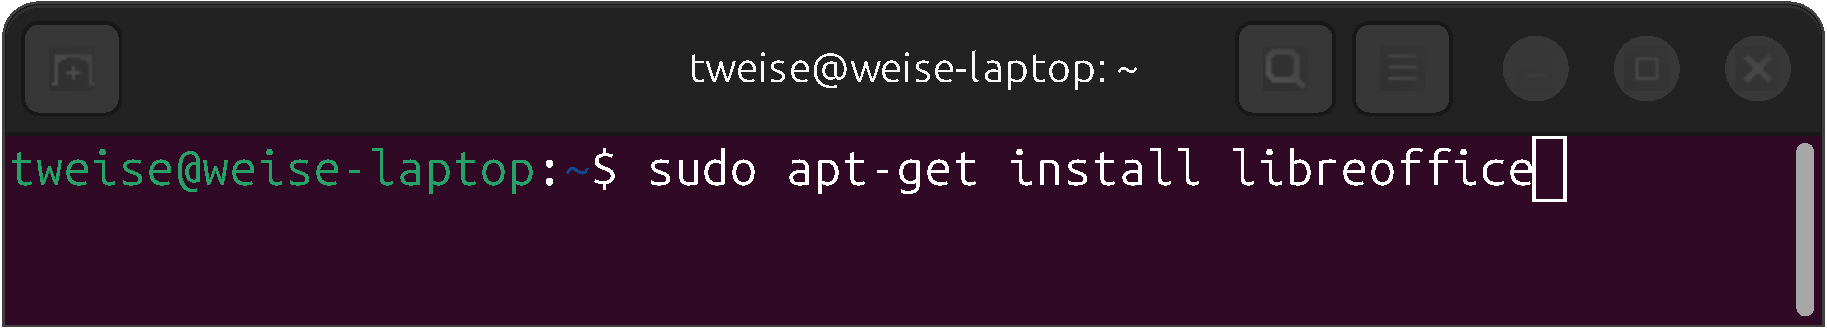
\includegraphics[width=0.7\linewidth]{\currentDir/installingLibreOfficeUbuntu7aptGet}}%
%
\floatRowSep%
%
\subfloat[][%
This requires \pgls{sudo} privileges, so we need to enter the super user password.%
\label{fig:installingLibreOfficeUbuntu8pw}%
]{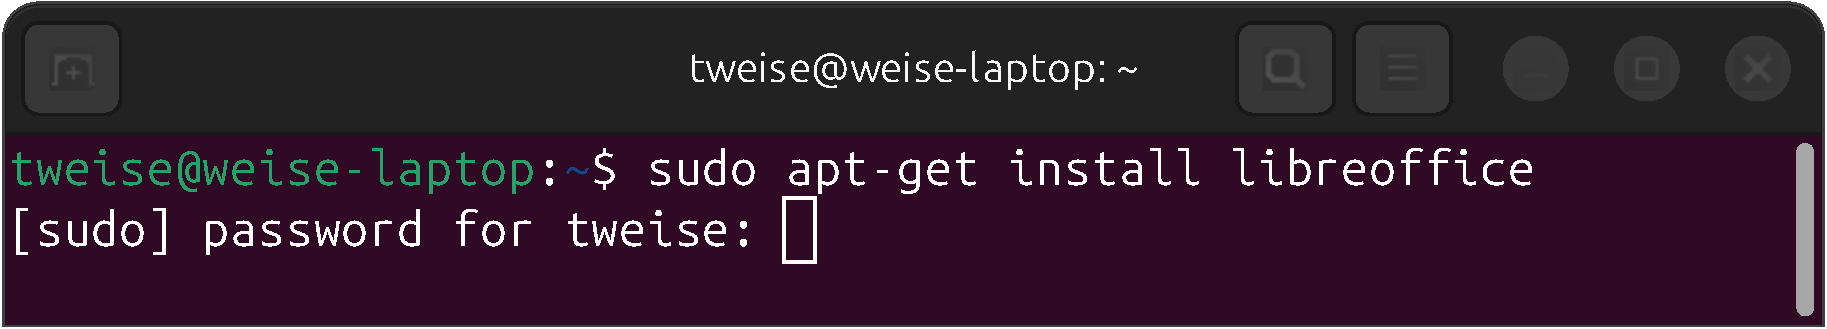
\includegraphics[width=0.7\linewidth]{\currentDir/installingLibreOfficeUbuntu8pw}}%
%
\floatRowSep%
%
\subfloat[][%
Now \libreoffice\ could be installed. %
On my system, it is already installed. %
So nothing happens.%
\label{fig:installingLibreOfficeUbuntu9already}%
]{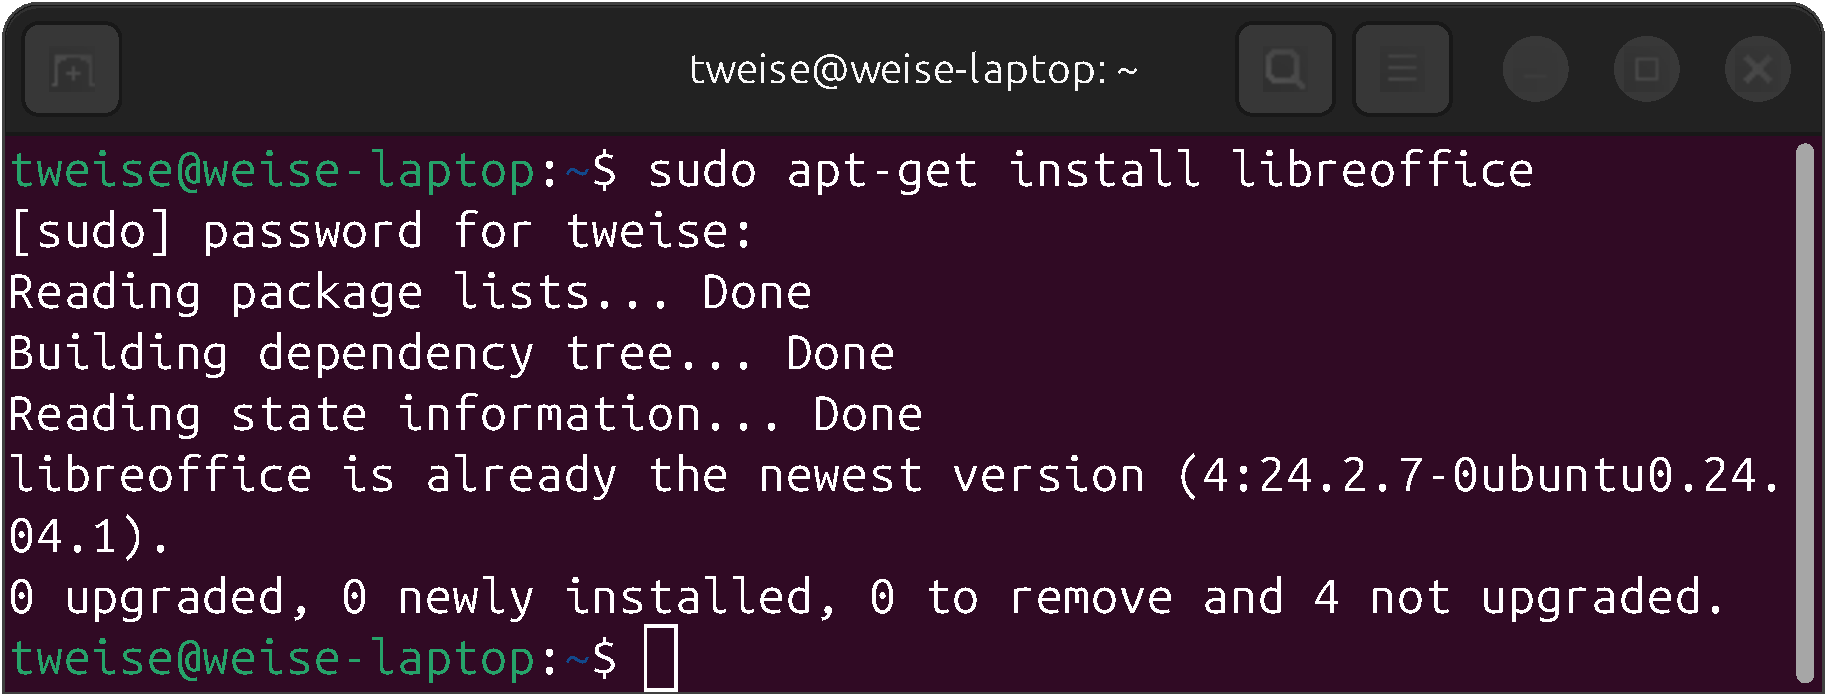
\includegraphics[width=0.7\linewidth]{\currentDir/installingLibreOfficeUbuntu9already}}%
%
\caption{Installing \libreoffice\ under \ubuntu.}%
\label{fig:installingLibreOfficeUbuntuC}%
\end{figure}%
%
If you are a user of \ubuntu\ \linux, then \libreoffice\ and, hence, \libreofficeBase, come already pre-installed on your machine.
You do not actually need to do anything.

To confirm that \libreoffice\ is indeed installed, we open
%
\FloatBarrier%
\endhsection%
%
